\documentclass[10pt]{article}
\usepackage[cp1251]{inputenc}
\usepackage[english]{babel}
\usepackage{url}
\usepackage{graphicx,DCCN2015_en}
\newcommand{\Rmnum}[1]{\expandafter\@slowromancap\romannumeral #1@}
\renewcommand{\Pr}{{\mathbf P}}

\makeatletter
\c@page=1 % Number will be set by publisher.
          
\makeatother


% Proper title, should be and will be capitalized
\title{Low-priority Queue Fluctuations in Tandem of Queuing Systems under Cyclic Control with Prolongations}
\author{V.~M.~Kocheganov$^1$, A.~V.~Zorine$^1$}
\company{$^1$ Departament of Applied Probability Theory, N.~I.~Lobachevsky State University of Nizhny Novgorod, Nizhny Novgorod, Russia}
\email{kocheganov@gmail.com, zoav1602@gmail.com}


%%%%%%%%%%%%%%%%%%%%%%%%%%%%%%%%

\begin{document}

\maketitle

%%%%%%%%%%%%%%%%%%%%%%%%%%%%%%%%%%%%%%%%%%%%%%%%%%%%%%%%%%%%%%
\begin{abstract}
A tandem of queuing systems is considered. Each system has a high-priority input flow and a low-priority input flow which are conflicting. In the first system, the customers are serviced in the class of cyclic algorithms. The serviced high-priority customers are transferred from the first system to the second one  with random delays and become the high-priority input flow of the second system. In the second system, customers are serviced in the class of cyclic algorithms with prolongations. Low-priority customers are serviced when their number exceeds a threshold. A mathematical model is constructed in form of a multidimensional denumerable discrete-time Markov chain. The recurrent relations for partial probability generating functions for the low-priority queue in the second system are found.

\keywords{tandem of controlling queuing systems, cyclic algorithm with prolongations, conflict flows, multidimensional denumerable discrete-time Markov chain}
\end{abstract}
%%%%%%%%%%%%%%%%%%%%%%%%%%%%%%%%%%%%%%%%%%%%%%%%%%%%%%%%%%%%%%


\section{Introduction}
Conflict traffic flows control at a crossroad is one of the classical problem of queuing theory. The problem has been solved for different classes of algorithms: the class of algorithms with a cyclic fixed rhythm, with renewals ("with a loop") with dynamic priorities, etc. However, several (two in our case) consecutive crossroads are of great interest, because in a real life situation after a car passes one highway intersection it finds itself at another one. In other words, output flow of the first intersection forms input flow of the second intersection. Hence, the second input flow no longer has simple probabilistic structure known a priori (for example, non-ordinary Poison process) and knowledge about service algorithm should be taken into account to deduce formation properties of the first output flow.

In \cite{k:z:02:2015} the problem of a tandem of two crossroads was carried out and rigorous probabilistic model was built. Description of the system is the following. At each of the road intersections, in addition to the high priority flow, there is the traffic flow "in the perpendicular direction" with lower priority. The service of the flows on the first intersection is supposed to be in the class of cyclic algorithms. In contrast the second intersection has cyclic algorithm with prolongations service type. Over and above, vehicles could not turn from one conflict direction to another. In this paper we continue the study of described problem and deepen in low priority flow of the second intersection investigation.


\section{The setting of the problem}

This section contains statement of the problem according to \cite{k:z:02:2015}. First of all the tandem is represented as queuing system to give generic formulation. In the end of the section system of two consecutive crossroads is given as simple example. Detailed mathematical model is built in next section.

Consider queuing system of the following type (see Fig.~\ref{SystemScheme}). 
\begin{figure}[h!]
   \centering
    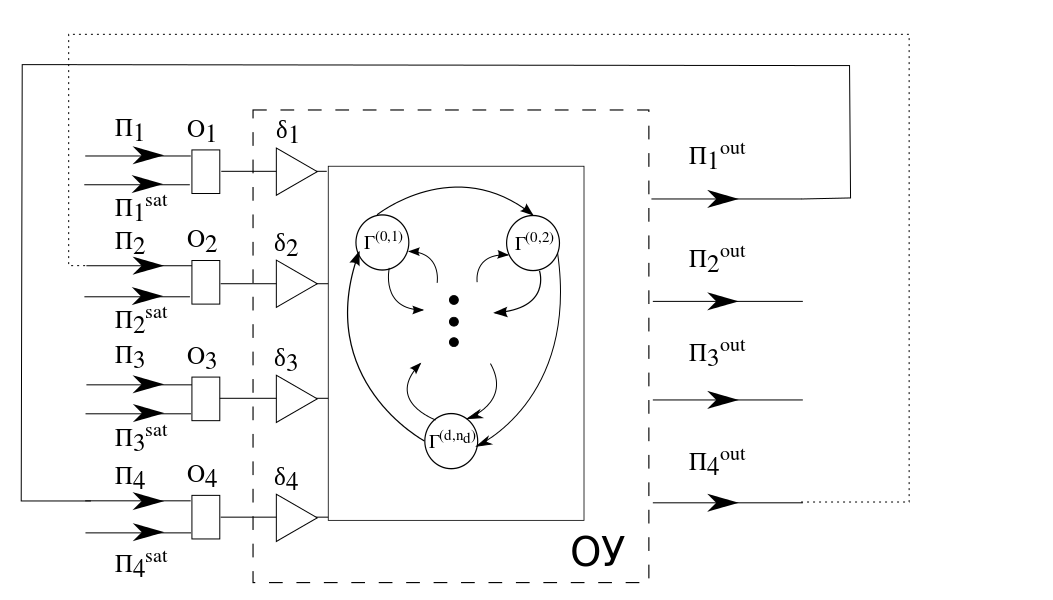
\includegraphics[width=\textwidth]{SystemScheme.png} % or {1.eps} in case of EPS format of the picture
    \caption {Structure scheme of queuing system}
    \label{SystemScheme}
\end{figure}
There are four input flows of customers coming into the system with one server. Customers from input flow $\Pi_j$ arrive to corresponding queue with an unbounded capacity, $j \in \{1,2,3,4\}$. For $j \in \{1,2,3\}$ discipline of the queue $O_j$ is FIFO (First In First Out). In other words, the earlier customer come to system the earlier it is serviced. Disciplie of the queue $O_4$ is described below. Input flows $\Pi_1$ and $\Pi_3$ are generated by external environment, which has only one state. Each of these flows is a nonordinary Poisson process. Denote $\lambda_1$ and $\lambda_3$ the intensity for the bulk arrival for the flows $\Pi_1$ and $\Pi_3$ respectively. Generating function of customer number in the bulk of flow $\Pi_j$ is
\begin{equation}
f_j(z) = \sum_{\nu=1}^{\infty} p_{\nu}^{(j)} z ^{\nu}, \quad j\in \{1,3\},
\label{GeneratingFunc}
\end{equation}
assuming it is finite for any $z\in \mathbb{C}$ such as $|z|<(1+\varepsilon)$, $\varepsilon>0$. Quantity $p_{\nu}^{(j)}$ is probability of event that customers number in a bulk of flow $\Pi_j$ is exactly $\nu$. Being serviced $\Pi_1$ customers come back to the system as $\Pi_4$ customers. $\Pi_4$ customers in turn after service come back to the system as $\Pi_2$ ones. Flows $\Pi_2$ and $\Pi_3$ are conflicting in the sense that customers arriving from different sources can't be serviced simultaneously in the same queuing system. This means that the problem can't be reduced to a corresponding problem with fewer input flows by merging the flows together.

Given positive integers $d$, $n_0$, $n_1$, $\ldots$, $n_d$, we introduce a finite set $\Gamma=\{\Gamma^{(k,r)} \colon k=0,1,\ldots,d; r=1,2,\ldots n_k\}$ of states in which server can be. At each state $\Gamma^{(k,r)}$ sever stays during time $T^{(k,r)}$. Define sets $\Gamma^{\mathrm{I}}$, $\Gamma^{\mathrm{II}}$, $\Gamma^{\mathrm{III}}$ and $\Gamma^{\mathrm{IV}}$ as follows. 
In state $\gamma \in \Gamma^{\mathrm{I}}$ only customers of queues $O_1$, $O_2$ and $O_4$ are serviced.
In state $\gamma \in \Gamma^{\mathrm{II}}$ only customers of queues $O_2$ and $O_4$ are serviced.
In state $\gamma \in \Gamma^{\mathrm{III}}$ only customers of queues$O_1$, $O_3$ and $O_4$ are serviced.
In state $\gamma \in \Gamma^{\mathrm{IV}}$ only customers of queues $O_3$ and $O_4$ are serviced.
The set $\Gamma$ is defined as union $\Gamma = \Gamma^{\mathrm{I}} \cup \Gamma^{\mathrm{II}} \cup \Gamma^{\mathrm{III}} \cup \Gamma^{\mathrm{IV}}$ disjoint sets. We will also need following sets in the future ${}^1\Gamma=\Gamma^{\mathrm{I}} \cup \Gamma^{\mathrm{III}}$, 
${}^2\Gamma=\Gamma^{\mathrm{I}} \cup \Gamma^{\mathrm{II}}$,
${}^3\Gamma=\Gamma^{\mathrm{III}} \cup \Gamma^{\mathrm{IV}}$. 

Server changes its state according to the following rule. We will call the set $C_k = \{\Gamma^{(k,r)} \colon r=1,2,\ldots n_k\}$  $k$-th cycle, $k=1$, $2$, $\ldots$, $d$. When $k=0$ state of the form 
$\Gamma^{(0,r)}$ is called prolongation state, $r=1$, $2$, $\ldots$, $n_0$. Denote $r \oplus_k 1 = r+1$ for $r<n_k$ and $r \oplus_k 1 = 1$ if $r=n_k$, $k = 0$, $1$, $\ldots$, $d$. In cycle $C_k$ we underline  subsets $C_k^{\mathrm{O}}$ input, $C_k^{\mathrm{I}}$ output and $C_k^{\mathrm{N}} = C_k \setminus (C_k^{\mathrm{O}} \cup C_k^{\mathrm{I}})$ neutral states. 
Then  after server was in state $\Gamma^{(k,r)} \in C_k\setminus C_k^{\mathrm{O}}$ it switches to the state $\Gamma^{(k,r \oplus_k 1)}$ of the same cycle $C_k$. 
After state $\Gamma^{(k,r)}$ in $C_k^{\mathrm{O}}$ server switches to the state $\Gamma^{(k,r \oplus_k 1)}$, if number of customers in the queue $O_3$ in switching moment greater than predetermined threshold $L$. 
In other case,  that is when number of customers in the queue $O_3$ lesser or equal than $L$, new state is prolongation one $\Gamma^{(0,r_1)}$, where $r_1=h_1(\Gamma^{(k,r)})$ and
$h_1(\cdot)$~--- given mapping of the set 
$\bigcup\limits_{k=1}^d C_k^{\mathrm{O}}$ to $\{1,2,\ldots, n_0\}$. 
After state $\Gamma^{(0,r)}$ the state of the same type $\Gamma^{(0,r_2)}$ is chosen, if number of customers in queue $O_3$ is lesser or equal than $L$, where $r_2=h_2(r)$ and $h_2(\cdot)$~--- given mapping of the 
set $\{1,2, \ldots, n_0\}$ to itself; in other case state of the form $\Gamma^{(k,r_3)} \in C_k^{\mathrm{I}}$ is on, where $\Gamma^{(k,r_3)}=h_3(r)$ and $h_3(\cdot)$~--- given mapping $\{1,2, \ldots, n_0\}$ to the set  $\bigcup\limits_{k=1}^d C_k^{\mathrm{I}}$. We assume that all prolongation states $\Gamma^{(0,r)}$ belong to the set ${}^2 \Gamma$, and  relations $C_k^\mathrm{O}\subset {}^2 \Gamma$ and $C_k^\mathrm{I}\subset {}^3 \Gamma$ are hold. We also assume that all the cycles have exactly one input and output state. And last assumption is that all the prolongation vertices form one cycle, that is we can put $h_2(r)=r\oplus_0 1$.

More formally server changes its states according to the following rule:
\begin{equation}
h(\Gamma^{(k,r)},y) = 
\begin{cases}
\Gamma^{(k,r \oplus_k 1)},& \quad \text{ if } (\Gamma^{(k,r)}\in C_k\setminus C_k^{\mathrm{O}}) \text{ or } (\Gamma^{(k,r)}\in C_k^{\mathrm{O}} \text{ \& } y>L);\\
%\Gamma^{(k,r \oplus_k 1)},& \quad \text{ if } \Gamma^{(k,r)}\in C_k^{\mathrm{O}} \text{ and } y>L;\\
\Gamma^{(0,h_1(\Gamma^{(k,r)}))},& \quad \text{ if } \Gamma^{(k,r)}\in C_k^{\mathrm{O}} \text{ and } y\leqslant L;\\
\Gamma^{(0,r \oplus_0 1)},& \quad \text{ if } k=0 \text{ and } y\leqslant L;\\
h_3(r),& \quad \text{ if } k=0 \text{ and } y > L.
\end{cases}
\label{hLaw}
\end{equation}

In general, service durations of different customers can be dependent and have different distributions. That is why instead of classic approach  which specifies distributions of every particular customer, saturation flows will be used. Such a flow $\Pi^{\mathrm{\text{sat}}}_j$, $j \in \{1,2,3,4\}$, 
is defined as virtual output flow given maximum loading of the server, and for $j\in \{1, 2, 3\}$ given also maximum loading of the corresponding queue. Saturation flow $\Pi^{\mathrm{\text{sat}}}_j$, $j\in \{1,2,3\}$, 
contains non-random number of customers $\ell_{k,r,j}$, serviced during time $T^{(k,r)}$, if server's state is $\Gamma^{(k,r)}$. Let $\mathbb{Z}_+$ be the set of non-negative integer numbers. Then given the fact, that queue $O_4$ contains $x \in \mathbb{Z}_+$ customers, saturation flow $\Pi^{\mathrm{\text{sat}}}_4$ is determined to contain all the $x$ customers.
Finally in the state $\Gamma^{(k,r)}$ every customer from queue $O_4$ with probability $p_{k,r}$ and independently of others ends servicing and come to queue $O_2$ of the flow $\Pi_2$. The customer of queue $O_4$ stay on up to the next round with probability $1-p_{k,r}$. On next round the picture is the same.

As we mentioned earlier in the end of the section we introduce real-life example of defined queuing system: tandem of two consecutive crossroads (Fig. \ref{crossroads}). 
\begin{figure}[h!]
   \centering
    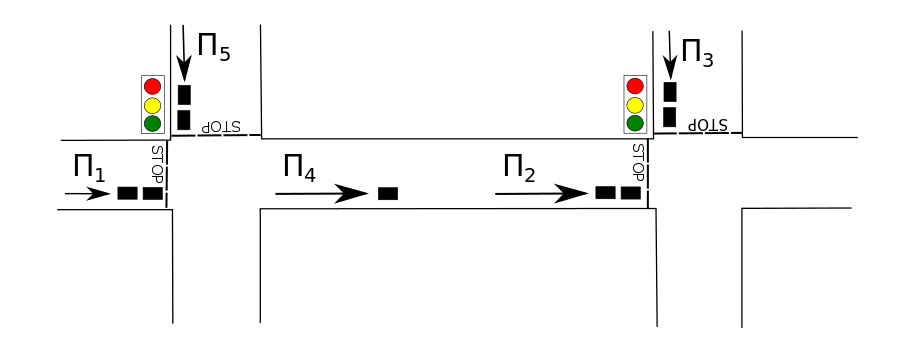
\includegraphics[width=\textwidth]{Crossroads.png} % or {1.eps} in case of EPS format of the picture
    \caption {Example: crossroads tandem}
    \label{crossroads}
\end{figure}
Flows of arriving cars play role of customer flows formed by external environment: conflicting flows $\Pi_1$ and $\Pi_5$ on the first crossroad; flow $\Pi_3$ on the second. Every car from flow $\Pi_1$, after passing first road intersection, comes to the queue $O_4$ of the flow $\Pi_4$. Whereupon the car arrives to the next road intersection with some probability ($p_{k,r}$ for the state $\Gamma^{(k,r)}$) or does not have time to do so and stays for another round. In case it has time it comes in queue $O_2$ and waits it's turn to pass it. Such system of two crossroads is an instance of more general queuing model described above.

\section{Mathematical model}
To build rigorous and complete probabilistic model of queuing system described in previous section cybernetic approach was used (see \cite{Fedotkin:1988}). Scheme of the controlling system was introduced on Fig.~\ref{SystemScheme}. There are following blocks presented on figure: 1) external environment with one state; 2) input poles of the first type --- input flows $\Pi_1$, $\Pi_2$, $\Pi_3$ and $\Pi_4$; 3) input poles of the second type --- saturation flows $\Pi^{\mathrm{\text{sat}}}_1$, $\Pi^{\mathrm{\text{sat}}}_2$, $\Pi^{\mathrm{\text{sat}}}_3$ and $\Pi^{\mathrm{\text{sat}}}_4$; 4) external memory --- queues $O_1$, $O_2$, $O_3$ and $O_4$; 5) device for external memory processing --- queue disciplines $\delta_1$, $\delta_2$, $\delta_3$ and $\delta_4$; 6) internal memory --- server; 7)  device for internal memory processing --- state changing graph; 8) output poles $\Pi^{\mathrm{\text{out}}}_1$, $\Pi^{\mathrm{\text{out}}}_2$, $\Pi^{\mathrm{\text{out}}}_3$ and $\Pi^{\mathrm{\text{out}}}_4$.
The coordinate of the block is its number on scheme.

To specify blocks information we introduce following variables and elements, along with their value ranges. To fix a discrete time scale consider the moments $\tau_0=0$, $\tau_1$, $\tau_2$, $\ldots$ when server changes its state. Denote $\Gamma_i$ from the set $\Gamma$ server's state during $\left(\tau_{i-1};\tau_i\right]$, $\varkappa_{j,i} \in \mathbb{Z}_+ $ number of customers in queue $O_j$ at the time $\tau_i$, $\eta_{j,i} \in \mathbb{Z}_+$ number of customers, came to the queue $O_j$ from the flow $\Pi_j$ during $\left(\tau_{i};\tau_{i+1}\right]$, $\xi_{j,i} \in \mathbb{Z}_+$ number of customers in the saturation flow $\Pi^{\mathrm{\text{sat}}}_j$ during $\left(\tau_{i};\tau_{i+1}\right]$, $\overline{\xi}_{j,i}\in \mathbb{Z}_+$ number of actually serviced customers in the flow $\Pi_j$ during $\left(\tau_{i};\tau_{i+1}\right]$, $j\in \{1,2,3,4\}$.

Server changes it's state according to the following rule:
\begin{equation}
\Gamma_{i+1}=h(\Gamma_i,\varkappa_{3,i}),
\label{gammaFunc}
\end{equation}
where mapping $h(\cdot,\cdot)$ is determined by \eqref{hLaw}.
To define a duration $T_{i+1}$ of the server state for time interval $\left(\tau_{i};\tau_{i+1}\right]$ it's handy to use mapping $h_T(\cdot,\cdot)$:
\begin{equation*}
T_{i+1}=h_T(\Gamma_i,\varkappa_{3,i})= T^{(k,r)},\quad  \text{ where } \Gamma^{(k,r)}=\Gamma_{i+1}=h(\Gamma_i,\varkappa_{3,i}).
%\label{timeLaw}
\end{equation*}
Functional relation
\begin{equation}
\overline{\xi}_{j,i}=\min\{\varkappa_{j,i}+\eta_{j,i},\xi_{j,i}\}, \quad j\in \{1,2,3\},
\label{saturationEq}
\end{equation}
between $\overline{\xi}_{j,i}$ and $\varkappa_{j,i}$, $\eta_{j,i}$, $\xi_{j,i}$ implements service strategy. Further since
\begin{equation*}
\varkappa_{j,i+1}=\varkappa_{j,i}+\eta_{j,i}-\overline{\xi}_{j,i}, \quad  j\in \{1,2,3\},
\end{equation*}
and due to \eqref{saturationEq} it follows that 
\begin{equation}
\varkappa_{j,i+1}=\max\{{0,\varkappa_{j,i}+\eta_{j,i}-\xi_{j,i}}\}, \quad j\in \{1,2,3\}.
\label{queuesFunc}
\end{equation}

The setting of the problem (see also structure scheme on Fig.~\ref{SystemScheme}) implies these relations for flow $\Pi_4$:
\begin{equation}
\eta_{4,i} = \min\{\xi_{1,i}, \varkappa_{1,i}+\eta_{1,i}\}, \quad \varkappa_{4,i+1}=\varkappa_{4,i}+\eta_{4,i}-\eta_{2,i}, \quad \xi_{4,i} = \varkappa_{4,i}.
\label{FourthFunc}
\end{equation}

Non-local description of the input and saturation flows involves specification of some particular features of conditional distributions of highlighted discrete components $\eta_i=(\eta_{1,i},\eta_{2,i}, \eta_{3,i}, \eta_{4,i})$ and $\xi_i=(\xi_{1,i}, \xi_{2,i}, \xi_{3,i}, \xi_{4,i})$ of marked point processes $\{(\tau_i, \nu_i, \eta_i); i\geqslant 0\}$ and $\{(\tau_i, \nu_i, \xi_i); i\geqslant 0\}$ given fixed label value $\nu_i = (\Gamma_i;\varkappa_i)$, where $\varkappa_i=(\varkappa_{1,i},\varkappa_{2,i},\varkappa_{3,i},\varkappa_{4,i})$. 
Let $\varphi_1(\cdot,\cdot)$ and $\varphi_3(\cdot,\cdot)$ be defined from decompositions 
\begin{equation*}
\sum_{\nu=0}^{\infty} z^\nu\varphi_j(\nu,t) = \exp\{\lambda_j t (f_j(z)-1)\},
\end{equation*}
where $f_j(z)$ are defined in \eqref{GeneratingFunc}, $j \in \{1,3\}$. Function $\varphi_j(\nu,t)$ defines probability of coming $\nu=0$, $1$, $\ldots$ customers of the flow $\Pi_j$ during time $t \geqslant 0$. If $\nu < 0$ value of $\varphi_j(\nu,t)$ is set to zero. Function $\psi(\cdot,\cdot,\cdot)$ is defined by formula

\begin{equation*}
\psi(k;y,u)=C_y^k u^k (1-u)^{y-k}.	
\end{equation*}
Semantically $\psi(k;y,u)$ is a probability of coming $k$ customers from flow $\Pi_2$ given $y$ customers in queue $O_4$ and $\Gamma^{(k,r)}$ as a state of the server, such that $u=p_{k,r}$. If condition $ 0\leqslant k \leqslant y$ does not hold $\psi(k;y,u)$ is set to zero.

Let $a=(a_1, a_2, a_3, a_4) \in \mathbb{Z}_+^4$ and $x=(x_1, x_2, x_3, x_4) \in \mathbb{Z}_+^4$. Then the setting of the problem implies that given fixed label value $\nu_i=(\Gamma^{(k,r)}; x)$ probability $\varphi(a,k,r,x)$ of following equations simultaneous holding $\eta_{1,i}=a_1$, $\eta_{2,i}=a_2$, $\eta_{3,i}=a_3$, $\eta_{4,i}=a_4$ is
\begin{equation}
\varphi_1(a_1,h_T(\Gamma^{(k,r)},x_3)) \times \psi(a_2,x_4, p_{\tilde{k},\tilde{r}}) \times \varphi_3(a_3,h_T(\Gamma^{(k,r)},x_3))
\times \delta_{a_4,\min{\{\ell(\tilde{k},\tilde{r},1), x_1+a_1}\}},
\label{conditionProbOne}
\end{equation}
where $\Gamma^{(\tilde{k},\tilde{r})}=h(\Gamma^{(k,r)},x_3)$ and $\delta_{i,j}$ is Kroneker's delta
\begin{equation*}
\delta_{i,j}=\begin{cases} 1, \quad \text{ if }i=j\\0, \quad \text{ if } i\neq j,
\end{cases}.
\end{equation*}
Let $b=(b_1, b_2, b_3, b_4) \in \mathbb{Z}_+^4$. The setting of the problem also implies that probability $\zeta(b, k, r, x)$  of following equations simultaneous holding $\xi_{1,i}=b_1$, $\xi_{2,i}=b_2$, $\xi_{3,i}=b_3$, $\xi_{4,i}=b_4$ given fixed label value $\nu_i=(\Gamma^{(k,r)}; x)$ is
\begin{equation}
\delta_{b_1,\ell(\tilde{k},\tilde{r},1)} \times \delta_{b_2,\ell(\tilde{k},\tilde{r},2)} \times 
\delta_{b_3,\ell(\tilde{k},\tilde{r},3)} \times \delta_{b_4,x_4}.
\label{conditionProbTwo}
\end{equation}

To gather all the assumptions made so far, we introduce below a theorem, which is described in more details in \cite{k:z:02:2015}. Specifically, theorem constructs probabilistic space on which all the mentioned random variables/elements and properties are consistent and therefore make mathematical sense.

\begin{thm}\label{thm1}
Let $\gamma_0=\Gamma^{(k_0,r_0)}\in \Gamma$ and $x^0=(x_{1,0},x_{2,0}, x_{3,0},x_{4,0})\in \mathbb{Z}_+^4$ be fixed.
Then there exists probabilistic space $(\Omega, {\cal F}, \Pr(\cdot))$ and random variables $\eta_{j,i}=\eta_{j,i}(\omega)$, $\xi_{j,i}=\xi_{j,i}(\omega)$, 	 $\varkappa_{j,i}=\varkappa_{j,i}(\omega)$ and random elements $\Gamma_i=\Gamma_i(\omega)$, $i\geqslant 0$, $j\in \{1, 2, 3, 4\}$, which are defined on this space, such that 1) equations $\Gamma_0(\omega) = \gamma_0$ and $\varkappa_0(\omega)=x^0$ hold; 2) propositions \eqref{gammaFunc}, \eqref{queuesFunc}, \eqref{FourthFunc} hold; 3) for any  $a$, $b$, $x^t=(x_{1,t},x_{2,t},x_{3,t},x_{4,t}) \in \mathbb{Z}_+^4$, $\Gamma^{(k_t,r_t)} \in \Gamma$, $t = 1, 2, \ldots$, conditional distribution of vectors  $\eta_i$, and $\xi_i$ has the form
\begin{equation}
\Pr \left(\{ \omega \colon \eta_i = a, \xi_i=b\} \left|\bigcap_{t=0}^{i}\{\omega\colon \Gamma_t=\Gamma^{(k_t,r_t)}, \varkappa_t=x^t\}\right.\right)=
\varphi(a,k_i,r_i,x^i)\times \zeta(b,k_i,r_i,x^i),
\label{ProbablititiesToProve}
\end{equation}
where mappings $\varphi(\cdot, \cdot, \cdot, \cdot)$ and $\zeta(\cdot, \cdot, \cdot, \cdot)$ are defined by \eqref{conditionProbOne} and \eqref{conditionProbTwo} respectively, $i \geqslant 0$.
\label{myTheorem}
\end{thm}

\section{Low-priority queue analysis}
The ultimate goal of the study is to analyse random sequence
\begin{equation}
\{(\Gamma_i, \varkappa_{1, i}, \varkappa_{2, i}, \varkappa_{3, i}, \varkappa_{4, i}); i \geqslant 0\}
\end{equation}
That is researcher is interested about it's Markove'ness, making classification of it's states, finding necessary and sufficient conditions on stationary distribution existence and finding important characteristics of such distribution. To come up with the solution of such a big problem it is easier to reduce problem into small ones. After the solutions for these issues is found researcher builds from them the solution for the main problem.

One of such small problems is analyses of sequence
\begin{equation}
\{(\Gamma_i, \varkappa_{3, i}); i \geqslant 0\}
\end{equation}
which includes low priority queue size $\varkappa_{3, i}$ (that is, size of queue $O_3$). This is a subsequence of $\{(\Gamma_i, \varkappa_{i}); i \geqslant 0\}$ that is why some of it's properties will be likely generalized on the entire sequence. Below we introduce several results which have been already obtained on the way of solving this sub-problem.

First result concerns Markov'ness of the subsequence.
\begin{thm}
Let $\Gamma_0=\Gamma^{(k,r)}\in \Gamma$ and $\varkappa_{3,0}=x_{3,0}\in \mathbb{Z}_+$ be fixed. Then sequence $\{(\Gamma_i, \varkappa_{3, i}); i \geqslant 0\}$ is homogeneous denumerable Markov chain.
\end{thm}

To continue we need following function.
For any $y_0$, $y$, $\tilde{y} \in \mathbb{Z}_+$ and $t \in \mathbb{R}$, $t\geqslant 0$ 
\begin{equation}
\widetilde{\varphi}_3(k,r,t,y,\tilde{y}) = (1-\delta_{\tilde{y},0}) \varphi_3(\tilde{y} + \ell(k,r,3)-y,t)  +\delta_{\tilde{y},0}\sum_{a=0}^{\ell(k,r,3)-y} \varphi_3(a,t),
\label{tildephi}
\end{equation}
where $k$ and $r$ such that $\Gamma^{(k,r)}\in \Gamma$.

In these notations following proposition is true.
\begin{thm}
Let $x_3$, $\tilde{x}_3\in \mathbb{Z}_+$ and $\Gamma^{(k,r)}$, $\Gamma^{(\tilde{k},\tilde{r})}=h(\Gamma^{(k,r)},x_3) \in \Gamma$. Then transition probabilities of  homogeneous denumerable Markov chain $\{(\Gamma_i, \varkappa_{3, i}); i \geqslant 0\}$ can be found from expressions
\begin{equation}
\Pr (\Gamma_{i+1}=\Gamma^{(\tilde{k},\tilde{r})},\varkappa_{3,i+1}=\tilde{x}|\Gamma_{i}=\Gamma^{(k,r)},\varkappa_{3,i}=x) 
= \widetilde{\varphi}_3(\tilde{k},\tilde{r},h_T(\Gamma^{(k,r)},x_3),x_3,\tilde{x}_3),
\label{transitionToProve:three}
\end{equation}
\end{thm}

Last theorem gives insight on what states of the chain $\{(\Gamma_i, \varkappa_{3, i}); i \geqslant 0\}$ are important. To make complete classification, we introduce sets
\begin{equation*}
\begin{aligned}
S^3_{0,r} = & \{(\Gamma^{(0,r)},x_3) \colon x_3\in Z_+, L \geqslant x_3 > L - \max\limits_{k=1, 2, \ldots, d}\{\sum_{t=0}^{n_k} \ell_{k,t,3}\}\}, \quad 1 \leqslant r \leqslant n_0, \\
S^3_{k,r} = & \{(\Gamma^{(k,r)},x_3) \colon x_3\in Z_+, x_3 > L - \sum_{t=0}^{r-1} \ell_{k,t,3}\} \}, \quad 1 \leqslant k \leqslant d, \quad 1 \leqslant r \leqslant n_k.
\end{aligned}
\end{equation*}

\begin{thm}
The set of important states of the Markov chain $\{(\Gamma_i, \varkappa_{3, i}); i \geqslant 0\}$  consists of sets $\bigcup\limits_{1 \leqslant r \leqslant n_0}S^3_{0,r}$ and $\bigcup\limits_{\substack{1 \leqslant k \leqslant d\\ 1 \leqslant r \leqslant n_k}} S^3_{k,r}$.
\end{thm}

At the end of this article we give result which is principle in finding necessary and sufficient conditions on stationary distribution existence of chain $\{(\Gamma_i, \varkappa_{3, i}); i \geqslant 0\}$.

Denote for $\gamma \in \Gamma$ and $x_3 \in Z_+$
\begin{equation}
Q_{3,i}(\gamma,x) = \Pr(\Gamma_{i}=\gamma, \varkappa_{3,i}=x_3).
\end{equation}
Suppose $k$ and $r$ such that $\Gamma^{(k,r)}\in \Gamma$. Partial generation functions are defined as follows:
\begin{align*}
\mathfrak{M}^{(i)}(k,r,v) &= \sum_{w=0}^{\infty} Q_{3,i}(\Gamma^{(k,r)},w) v^w,\\
\Phi^{(i)}(k,r,v) &= q_{k,r}(v) \sum_{x_3=0}^{\infty} \sum_{\gamma \in H_{-1}(\Gamma^{(k,r)},x_3)} Q_{3,i}(\gamma,x_3) v^{x_3},
\end{align*}
where
\begin{equation*}
q_{k,r}(v) = v^{-\ell(k,r,3)}\sum_{w=0}^{\infty} \varphi_3(w,T^{(k,r)})v^w.
\end{equation*}

\begin{thm}
Let $\tilde{\gamma}=\Gamma^{(\tilde{k},\tilde{r})} \in \Gamma$. The following recurrent by $i \geqslant 0$ relations take place for partial generation functions of Markov chain $\{(\Gamma_i, \varkappa_{3, i}); i \geqslant 0\}$:
\begin{multline}
\mathfrak{M}^{(i+1)}(\tilde{k},\tilde{r},v) = \Phi^{(i)}(\tilde{k},\tilde{r},v)+\sum_{x_3=0}^{\ell(\tilde{k},\tilde{r},3)}\sum_{\gamma \in H_{-1}(\tilde{\gamma},x_3)} Q_{3,i}(\gamma,x_3) \sum_{a=0}^{\ell(\tilde{k},\tilde{r},3) - x_3} \varphi_3(a,T^{(\tilde{k},\tilde{r})}) - \\
- \sum_{x_3=0}^{\ell(\tilde{k},\tilde{r},3)}  \sum_{\gamma \in H_{-1}(\tilde{\gamma},x_3)} Q_{3,i}(\gamma,x_3) v^{x_3-\ell(\tilde{k},\tilde{r},3)}  \sum_{w=0}^{\ell(\tilde{k},\tilde{r},3) + 1 -x_3}\varphi_3(w,T^{(\tilde{k},\tilde{r})}) v^w.
\label{markk_proiz}
\end{multline}
\end{thm}



\begin{thebibliography}{99}
\bibitem{k:z:02:2015}  %% citation code
Kocheganov V.~M., Zorine A.V. Probabilistic model of tandem of queuing systems under cyclic control with prolongations ~// Probability theory, stochastic processes, mathematical statistics and applications, Minsk, 2015. -- P.~94-99. (Russian)

\bibitem{Fedotkin:1988} Fedotkin M.~A. Optimal control for conflicting flows and marked point processes with an iso-
lated discrete component. I, Litovsk. Mat. Sb. 28, 1988, no. 4, P.~783-794. (Russian)

\end{thebibliography}
\end{document}
